\chapter{Implementation}
\label{chapter:implementation}

% This chapter should include design choices for my implementation. For
% example choices taken for generating relevant data for test users
% and a computational sound method for doing so. As JavaScript in browsers are
% quite inefficient it will probably be necessary to persist data at a server
% in some sort of cache. The clients could then get this data by invoking a
% single request. The result could for instance be JSON serialized. Scraping
% of such data is probably done more efficient and safer at the server side
% since multiple XMLHttpRequests in the clients for scraping and parsing could
% prove to be quite computational expensive.

As we've seen in 
\sectionref{building.on.top.of.the.web}
it's possible to build applications on top of existing web sites by creating
transparent prototype implementations. This chapter starts with an account of
what kind of navigation system we wanted to build, goes on to describe why we
decided on such navigational designs, and concludes with an explanation of how
the implementation was built\dash{}the ingredients of our implementation.

\section{Design}

% no new data. making existing data more readily available.

\section{Process}
% Prototype, exploratory
% TDD, BDD

\subsection{Prototyping}

A \term{prototype} is an early version of an application that are used for
finding out more about the problem at hand and it's possible solutions
\citep[p.~409]{sommerville07}.
The software developed for our research on social navigation fits these
characteristics. It's not supposed to be used after it's behavior is
evaluated. For that it's to inefficient and relies on specific web browser
environments and extensions. This does not mean that the prototype can't have
impact on how \urort{} evolves in the future. If our evaluation favors our
design decisions the developers of \urort{} might take advantage of such
potential improvements in their web site design.

\citet[pp.~409--410]{sommerville07} explains that a prototype can be used for
\begin{inparaenum}[(i)]
  \item gathering more sound requirements from users during a
    requirements phase,
  \item evaluating the feasibility of a proposed design during a
    design phase, and
  \item testing the final system by verifying it against the prototype.
\end{inparaenum}
We're following his second example of prototype usage by making a prototype
for what we believe to be a sound social navigation design. This is then
evaluated. If time permitted (sadly one has limited time and resources
available during master thesis research) the results of such an evaluation
could be input in a new design process and a new prototype system.

As \citet[p.~114]{mcconnell04} explains prototyping can mean different things
based on context. Often it's used to explain systems where one writes the
least amount of code to get a solution and throw it all away when the design
question is answered. This is not our intention. We'll try to make the system
fully operational and make the code we author comprehensible and
valid. More precisely we're creating a \term{high-fidelity} prototype
\cite[p.~78]{rudd96} with a robust architecture.

\subsection{Testing}


\section{Architecture}

Our implementation basically needs to do two things:

\begin{enum}
  \item Collect existing data from various places on the \urort{} web site.
  \item Display this data in existing web pages on the \urort{} web site in
    a way that we hope will enhance navigation.
\end{enum}

We decided to use a server--client architecture so that we could offload some
of the more computationally expensive operations off the client and onto a
dedicated server. Another benefit of such an architecture is that it allows us
to cache data globally\dash{}shared by all clients. Therefore data collection
is handled on the server side, while data display obviously is handled on
the client side.

\subsection{Server--Client Architecture}
% Describe possible increased performance with server/client side from
% literature.

% similar architecture: nishimoto06

\subsection{Asyncronous Requests}

In the traditional style of \abbr{AJAX} applications we request information on
the client side of our prototype asyncronous. This means that requests
handeled by the \code{XMLHttpRequest} object
% more about asyncronous versus syncronous:
% http://yuiblog.com/blog/2006/04/04/synchronous-v-asynchronous
%
% cite stamey06 about network latency, not needing to fetch a whole page,
% AJAX request independent of HTTP requests, etc.

With all the pieces in place of our third party software puzzle described in
\chapterref{selection.of.third.party.software}
we present a high level view of the architecture, from the client to the
server, in
\figureref{fig.prototype.architecture}.

\begin{figure}
  \begin{whole}
    \centering
    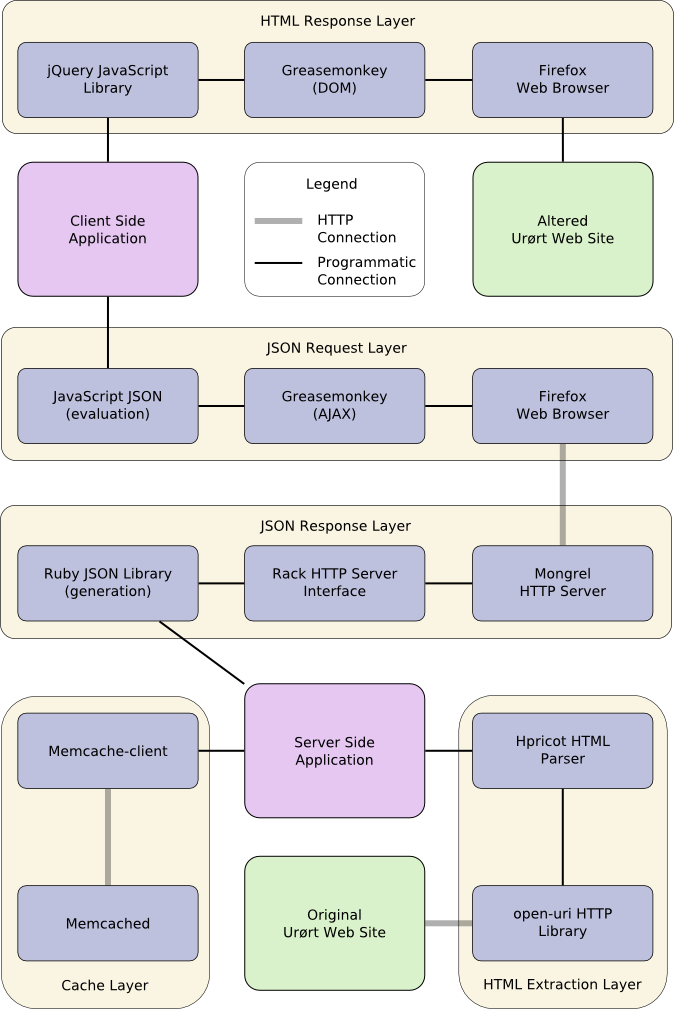
\includegraphics[width=0.9\wholewidth]{fig_prototype_architecture}
    \caption[Prototype Architecture]{
      High level view of the overall prototype architecture.
    }
    \label{figure:fig.prototype.architecture}
  \end{whole}
\end{figure}

% write about the cache and what is done on a \term{cache miss}. Also give
% reasons for \term{time to live}.

\subsection{Modularization}

% ruby modules, classes, separate files and directories
% packaged up with rubygems to make exchange and installation of the software
% easier.
% javascript packaging necessary? only downloaded once. gzip compression not
% an option. maybe minifying or deep packaging processes?

\subsection{Data Structure}
% the structure of our persistent data
